\documentclass{article}

%
% 引入模板的style文件
%
\usepackage{homework}

\setCJKmainfont{SimSun}[AutoFakeBold] %宋体加粗
\setCJKsansfont{SimHei}[AutoFakeBold] %黑体加粗


\usepackage{minted} %配合minted宏包进行好看的高亮
\usepackage{currfile} %配合minted宏包进行好看的高亮
\usepackage{caption} %配合minted宏包进行好看的高亮
\usepackage{tcolorbox} %配合minted宏包进行好看的高亮
\usepackage{xcolor} %配合minted宏包进行好看的高亮
\tcbuselibrary{skins} %配合minted宏包进行好看的高亮
\tcbuselibrary{minted} %配合minted宏包进行好看的高亮
\usemintedstyle{paraiso-dark} %配合minted宏包进行好看的高亮
\usepackage{framed} 
\usepackage{amsmath}


%
% 封面
%


\title{
	
\includegraphics[width=0.6\textwidth]{images/title/ucas_logo 1.pdf}\\
    \vspace{1in}
    \textmd{\textbf{\hmwkClass}}\\
	\textmd{\Large{\textbf{\hmwkClassID}}}\\
    \textmd{\textbf{\hmwkTitle}}\\
    \normalsize\vspace{0.1in}\large{\hmwkCompleteTime }\\
    \vspace{0.1in}\large{\textit{\hmwkClassInstructor\ }}\\
    \vspace{1in}
	
\includegraphics[width=0.25\textwidth]{images/title/Cyber.jpg}\\
	\vspace{1in}
}

\author{
	\hmwkAuthorName \\ 
	\hmwkAuthorStuID \\
	\hmwkAuthorInst \\
	\hmwkAuthorzhuanye \\
	\hmwkAuthorfangxiang
	}
\date{}

\renewcommand{\part}[1]{\textbf{\large Part \Alph{partCounter}}\stepcounter{partCounter}\\}


%
% 正文部分
%
\begin{document}


\maketitle


%\include{chapters/ch01}
%\include{chapters/ch02}
%\include{chapters/ch03}
%\include{chapters/ch04}
%\include{chapters/ch05}


\pagebreak



\begin{homeworkProblem}
	假设对称旅行商问题的邻接矩阵如下所示, 试用优先队列式分枝限界算法给出最短环游. 画出状态空间树的搜索图, 并说明搜索过程.
	$$
	\left( \begin{matrix}
		\infty&		20&		30&		10&		11\\
		&		\infty&		16&		4&		2\\
		&		&		\infty&		6&		7\\
		&		&		&		\infty&		12\\
		&		&		&		&		\infty\\
	\end{matrix} \right)
	$$
	\begin{figure}[H]
		\centering
		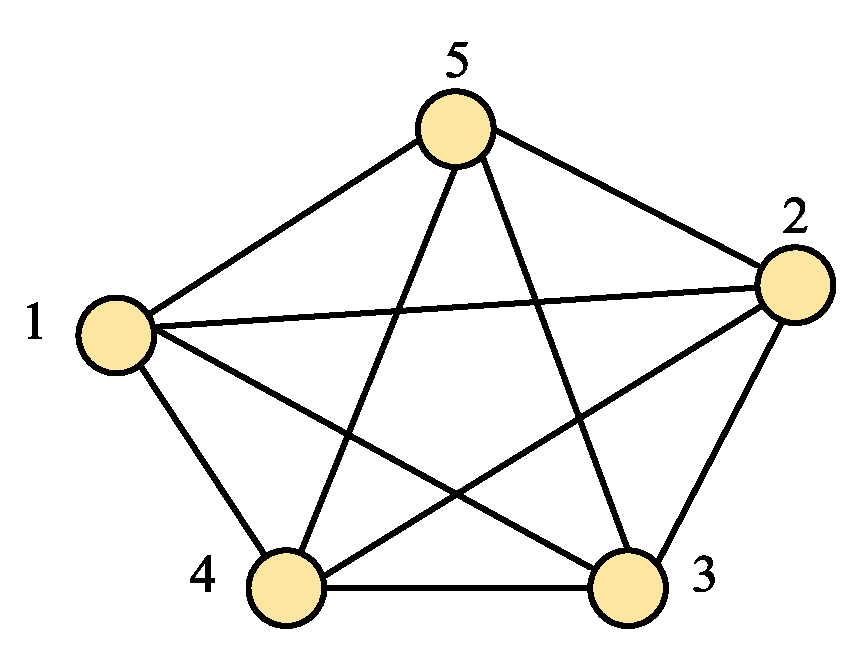
\includegraphics[width=0.3\textwidth]{images/title/旅行商问题.pdf}
		\caption{旅行商问题}
		\label{fig:旅行商问题}
	\end{figure}
	\solution 状态空间树的搜索图如下图\ref{fig:解空间树搜索图}中所示:
	\begin{figure}[H]
		\centering
		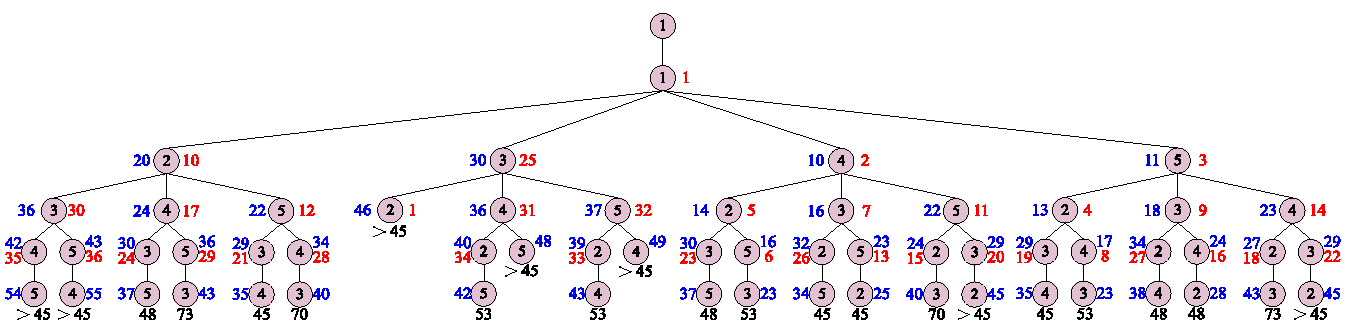
\includegraphics[width=1.0\textwidth]{images/title/解空间树搜索图.pdf}
		\caption{解空间树搜索图}
		\label{fig:解空间树搜索图}
	\end{figure}
	图中圆圈内为顶点序号, 蓝色数字为该路径到该节点的总路程, 红色数字表示该节点的搜索序数. 从顶点1开始搜索, 将其4个儿子节点放入队列. 然后优先访问队列中当前路程最小的节点, 再将它的儿子放入队列. 然后重复上述过程, 优先访问队列中当前路径最小的节点, 将其儿子放入队列. 第一个被访问到的叶子节点为1-4-2-5-3-1这条路径, 总路程为53, 记录当前最短路径. 之后若某节点的路径大于最短路程, 则不再搜索该节点的子树. 若某叶子节点的总路程小于当前最短路径, 则更新之. 如此搜索, 当访问到1-4-3-5-2-1这条路径的叶子节点时, 其总路程为$45<53$, 将45更新为当前最短路径, 继续搜索. 最后得出最短环游为1-2-5-3-4-1、1-4-3-2-5-1、1-4-3-5-2-1、1-5-2-3-4-1, 总路程均为45.
\end{homeworkProblem}


\pagebreak





\begin{homeworkProblem}
	最佳调度问题: 假设有$n $个任务要由$k $个可并行工作的机器来完成, 完成任务$i $需要的时间为$t_i$. 试设计一个分枝限界算法, 找出完成这$n $个任务的最佳调度, 使得完成全部任务的时间(从机器开始加工任务到最后停机的时间)最短.

	\solution \textbf{限界函数:} 将$n$个任务按照所需时间非递减排序, 得到任务序列$1,2,\cdots,n,$满足时间关系$t[1]<t[2]<\cdots<t[n]$. 将$n$个任务中的前$k$个任务分配给当前$k$个机器, 然后将第$k+1$个任务分配给最早完成已分配任务的机器, 依次进行, 最后找出这些机器最终分配任务所
	需时间最长的, 此时间作为分支限界函数. 如果一个扩展节点所需的时间超过这个已知的最优值, 则删掉以此节点为根的子树. 否则更新最优值.

	\textbf{优先级:} 哪台机器完成当前任务的时间越早, 也就是所有机器中最终停机时间越早, 优先级就越高, 即被选作最小堆中的堆顶, 作为扩展节点. 分支限界算法如下所示:
\begin{tcblisting}{listing engine=minted,boxrule=0.1mm,
colback=blue!5!white,colframe=blue!75!black,
listing only,left=5mm,enhanced,sharp corners=all,
overlay={\begin{tcbclipinterior}\fill[red!20!blue!20!white] (frame.south west)
rectangle ([xshift=5mm]frame.north west);\end{tcbclipinterior}},
minted language=c++,
minted style=tango,
minted options={fontsize=\small,breaklines,autogobble,linenos,numbersep=3mm}}
Node{
    int Path[n];
    int T[k];
    int Time;
    int length;
}
Proc BestDispatch(int n, int k, int t[]){
    Node Boot, X, P, result;
    int f;
    f = n * max(t[]);
    Boot.T[n] = {0};
    Boot.Time = 0;
    Boot.Path[n] = {0};
    Boot.length=0;
    AddHeap(Boot);
    while (!Heap.empty()) do {
        P = DeleteMinHeap();
        for i = 1 to k do {
            X = Newnode(P.Path[], P.T[], P.length + 1);
            X.Path[X.length] = i;
            X.T[i] = X.T[i] + t[X.length];
            X.Time = max(X.T[]);
            if X.length == n then {
                if X.Time < f then {
                    f = X.Time;
                    result = X;
                }
            }
            else {
                if X.Time < f then {
                    AddHeap(X);
                }
            }
        }
    }
}
end {BestDispatch}
\end{tcblisting}
\end{homeworkProblem}




\begin{homeworkProblem}
	\textbf{恰好覆盖问题:} 设给定有限集$A=\left\{ a_1,a_2,\cdots,a_n \right\}$和$A$的子集的集合$W=\left\{ S_1,S_2,\cdots,S_m \right\}$. 求子集$W$的子集$U$, 使得$U$中的子集都不相交且他们的并集等于$A$. 求满足条件的所有子集$U$.

	\solution 解向量为$\left( x_1,x_2,\cdots ,x_m \right) ,x_i=0,1$, 其中$x_i=1$当且仅当$S_i\in W$. 部分向量$(x_1,x_2,\cdots,x_k)$表示已经考虑了对$S_1,S_2,\cdots,S_k$的选择. $U$为当前所选择集合的并集.
	回溯算法如下所示:
	\begin{algorithm}[H]
		\begin{algorithmic}[1]
		\If{$k=m+1$}
			\State \Return;
		\EndIf
		\If{$|U+W(k)|=|U|+|W(k)|$}
			\State $X[k]=1$;
			\If{$|S+W(k)|=|A|$}
				\State \textbf{print} $X[\quad]$, \Return;
			\Else
				\State \textbf{Eaxtsetcover}$(U+W(k),k+1)$;
			\EndIf
		\EndIf
		\State $X[k]=0$;
		\State \textbf{Eaxtsetcover}$(U,k+1)$;
		\State \textbf{end \{Eaxtsetcover\}}
		\end{algorithmic}
		\caption{\textbf{Eaxtsetcover}$(U,k)$}
		\label{alg:Eaxtsetcover}
	\end{algorithm}
\end{homeworkProblem}





\begin{homeworkProblem}
	分派问题: 给$n$个人分派$n$件工作, 给第$i$人分派第$j$件工作的成本是$C(i,j)$, 试用分枝限界法求成本最小的工作分配方案.

	\solution 设$n$个人的集合是$\left\{ 1,2,\cdots,n \right\}$, $n$项工作的集合是$\left\{ 1,2,\cdots,n \right\}$, 每个人恰好1项工作. 于是有
	$$\text{把工作}j\text{分配给}i\Leftrightarrow x_i=j,\quad i,j=1,2,\cdots n
	$$

	设解向量为$X=\left< x_1,x_2,\cdots ,x_n \right>	$, 分配成本为$\displaystyle C\left( X \right) =\sum_{i=1}^n{C\left( i,x_i \right)}	$. 搜索空间是排列树. 部分向量$\left< x_1,x_2,\cdots ,x_k \right> $表示已经考虑了人$1,2,\cdots,k$的工作分配. 节点分支的约束条件为:$$x_{k+1}\in \left\{ 1,2,\cdots ,n \right\} \backslash \left\{ x_1,x_2,\cdots ,x_k \right\} 
	$$

	可以设立代价函数:$$F\left( x_1,x_2,\cdots ,x_k \right) =\sum_{i=1}^k{C\left( i,x_i \right)}+\sum_{i=k+1}^n{\text{min} \left\{ C\left( i,t \right) :t\in \left\{ 1,2,\cdots ,n \right\} \backslash \left\{ x_1,x_2,\cdots ,x_k \right\} \right\}}
	$$
	界$B$是已得到的最好可行解的分配成本. 如果代价函数大于界, 则剪枝并回溯. 可用优先队列分支限界算法, 以
	$F$最小优先扩展. 根节点有$n$个儿子$x_1=1,2,\cdots n$, 儿子节点有$n-1$个儿子$x_2=2,3,\cdots n$; $x_2=1,3,4,\cdots n;\cdots $. 算法描述如下, 其时间复杂度为$O(n\cdot n!)$.
\begin{tcblisting}{listing engine=minted,boxrule=0.1mm,
colback=blue!5!white,colframe=blue!75!black,
listing only,left=5mm,enhanced,sharp corners=all,
overlay={\begin{tcbclipinterior}\fill[red!20!blue!20!white] (frame.south west)
rectangle ([xshift=5mm]frame.north west);\end{tcbclipinterior}},
minted language=c++,
minted style=tango,
minted options={fontsize=\small,breaklines,autogobble,linenos,numbersep=3mm}}
Node{
    int Path[n];
    int work[n];
    int T[k];
    int Time;
    int length;
}
Proc BestDispatch(int n, int k, int t[]){
    Node Boot, X, P, result;
    int f;
    f = n * max(t[]);
    Boot.T[n] = {0};
    Boot.Time = 0;
    Boot.Path[n] = {0};
    Boot.length=0;
    AddHeap(Boot);
    while (!Heap.empty()) do {
        P = DeleteMinHeap();
        for i = 1 to n do {
            if(work[i] == 0) {
                X = Newnode(P.Path[], P.T[], P.length + 1);
                work[i] = 1;
            }
            X.Path[X.length] = i;
            X.T[i] = X.T[i] + t[X.length];
            X.Time = max(X.T[]);
            if X.length == n then {
                if X.Time < f then {
                    f = X.Time;
                    result = X;
                }
            }
            else {
                if X.Time < f then {
                    AddHeap(X);
                }
            }
        }
    }
}
end {BestDispatch}
\end{tcblisting}
\end{homeworkProblem}

\pagebreak


\begin{homeworkProblem}
	如图\ref{fig:Latin方}所示, 一个4阶Latin方是一个$4\times 4$的方格, 在它的每个方格内填入$1,2,3$或4, 并使得每个数字在每行、每列都恰好出现一次. 用回溯法求出所有第一行为1,2,3,4的所有4阶Latin方. 将每个解的第2行到第4行的数字从左到右写成一个序列. 如图\ref{fig:Latin方}中的解是$\left<3,4,1,2,4,3,2,1,2,1,4,3\right>$. 给出所有可能的4阶Latin方.
	\begin{figure}[H]
		\centering
		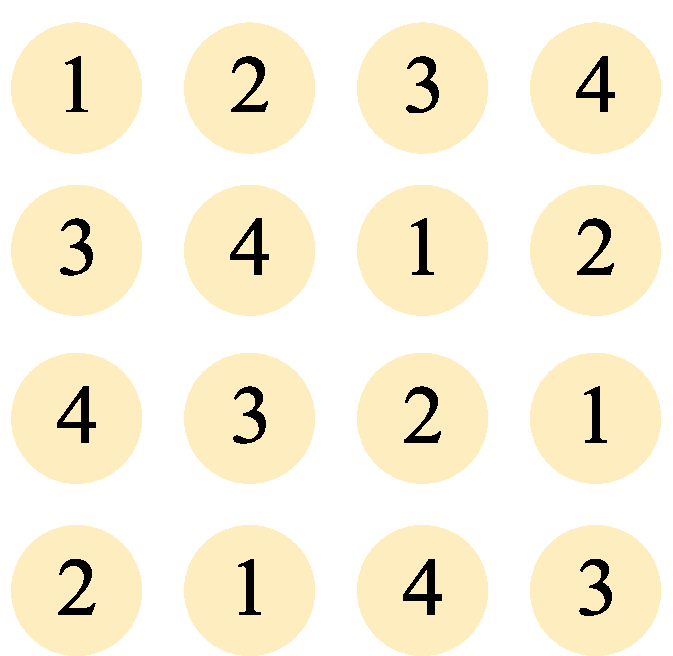
\includegraphics[width=0.2\textwidth]{images/title/Latin方.pdf}
		\caption{Latin方}
		\label{fig:Latin方}
	\end{figure}
	\solution 解向量为$X[4][4]$, 约束条件: 同行、同列不能相等. 因此回溯算法设计如下:
\begin{tcblisting}{listing engine=minted,boxrule=0.1mm,
colback=blue!5!white,colframe=blue!75!black,
listing only,left=5mm,enhanced,sharp corners=all,
overlay={\begin{tcbclipinterior}\fill[red!20!blue!20!white] (frame.south west)
rectangle ([xshift=5mm]frame.north west);\end{tcbclipinterior}},
minted language=c++,
minted style=tango,
minted options={fontsize=\small,breaklines,autogobble,linenos,numbersep=3mm}}
bool Latincheck(int X[4][4], int k, int row, int line) {
    for(int i = 0; i < row; i++) {
        if(X[i][line] == k) return false;
    }
    for(int j = 0; j < line; j++) {
        if(X[row][j] == k) return false;
    }
    return true;
}
void LatinMatrix(int X[4][4], int row, int line) {
    if(row == 3 && line == 3) {
        for(int i = 0; i < 4; i++)
            for(int j = 0; j < 4; j++)
                cout << X[i][j] << " ";
        return ;
    }
    else {
        for(int color = 1; color <= 4; color++) {
            if(Latincheck(X, color, row, line)) {
                X[row][line] = color;
                if(line < 3) LatinMatrix(X, row, line + 1);
                else if (line == 3 && row != 3) LatinMatrix(X, row + 1, 0);
            }
        }
    }
}
\end{tcblisting}
\end{homeworkProblem}



% 引用文献
\bibliographystyle{unsrt}  % unsrt:根据引用顺序编号
\bibliography{refs}


\end{document}
